\selectlanguage{italian}
\chapter{Svolgimento del Project Work}
\fancyhead[L]{Svolgimento del Project Work}

\section{La metodologia agile}
\begin{multicols}{2}
	Durante le prime fasi di confronto con Claudio Carbonaro e le prime visite in azienda, è stato deciso che la metodologia applicata sarebbe stata basata sulle tecniche agili giapponesi basate sulla filosofia di Toyota. Questa metodologia è stata considerata efficace per l’azienda data la sua semplicità di applicazione e snellezza.

	La prima difficoltà affrontata è stata convincere l’azienda dell’efficacia di queste tecniche. Le metodologie agili giapponesi utilizzano sistemi semplici e accessibili a tutti, come i post-it e danno meno importanza a soluzioni complicate e costose come i sistemi informativi. Questa differenza culturale ha generato inizialmente una certa resistenza da parte dell’azienda che è abituata a pratiche più convenzionali.

	Vista l’opposizione all’adottare soluzioni culturalmente molto lontane dalla prassi occidentale è stato deciso di mantenere le logiche, ma espanderle col supporto di strumenti informativi semplici come fogli Excel e OneNote.
	Nonostante l’azienda non sia dotata di un software di pianificazione della produzione ne è infatti stata sconsigliata l’adozione almeno per il momento.
	In assenza di logiche opportune infatti, questi programmi rischiano di essere mal utilizzati e non portare valore aggiunto all’azienda.
	È stato quindi deciso che l'azienda adotterà prima le logiche proposte. Se queste si dimostreranno efficaci, verranno successivamente adottati software di supporto se ritenuti necessari dall’azienda. Questa implementazione graduale permetterà di verificare l’efficacia delle nuove metodologie senza gravare l’azienda con costi immediati e senza creare ulteriore resistenza al cambiamento.

\section{Value Stream Map}
	La prima logica di lean manufacturing adottata è stata la rappresentazione della “value stream” dell’azienda, permettendo a me e a Claudio di comprendere il ciclo produttivo di Montagna, dalla ricezione dell’ordine alla consegna.

	L’obiettivo della stesura di una value stream map è quello di evidenziare eventuali sprechi e rimuoverli, portando a una maggiore efficienza e rendendo le operations più snelle, facilitando così anche la riduzione di scarti e problemi di qualità.

	Uno degli aspetti che è risultato piuttosto evidente fin da subito è che tra le fasi svolte non esistono dei gate di riesame che bloccano le fasi a valle se quella a monte non incontra determinati standard. Questo flusso continuo senza controlli intermedi porta a problemi di qualità e inefficienze, poiché i difetti possono propagarsi attraverso le varie fasi del processo produttivo.

	Per affrontare questa criticità, è stato suggerito di introdurre la stesura di una FMEA (Failure Mode and Effect Analysis) come strumento per garantire che il progetto sia conforme alle richieste del cliente e alle normative vigenti. Solo una volta condotta questa analisi la produzione può iniziare, garantendo standard progettuali elevati e che proteggano l’azienda da non conformità legate al design del prodotto.


\section{Analisi dei consuntivi}
	In parallelo al lavoro svolto con Claudio è stato ritenuto importante da Domenico lavorare sui pochi dati raccolti dall’azienda, che sono principalmente i consuntivi delle commesse svolte. Per fare ciò ho svolto un’analisi dei dati utilizzando R, che partendo dai file Excel estraesse ogni voce e il relativo valore, per cercare delle variabili che permettessero di discriminare tra le commesse andate bene e quelle andate male.

	\subsubsection{Analisi delle ore di lavoro}
	La prima analisi condotta ha riguardato il controllo delle ore usate per ogni singola attività rispetto al totale delle ore dedicate a una commessa. Ciò che è apparso evidente è stato come la distribuzione è molto simile anche tra commesse che hanno risultati molto diversi. Per tutte le commesse infatti, la percentuale di ore per fase era circa la seguente:
	\begin{itemize}
		\item Assemblaggio: Circa il 40\% del tempo totale di ogni commessa
		\item Taglio, piegatura e saldatura: Mediamente il 30\%
		\item Progettazione: Tra il 7\% e il 15\%, in base alla complessità delle richieste
		\item Altre attività: Lavorazioni meccaniche e attività di supporto, che occupano il resto del tempo
	\end{itemize}

	La mancanza di differenze sostanziali in termini di tempo tra commesse con buoni margini e commesse andate male suggerisce che non ci sono attività critiche che sovente ricevono rallentamenti e rilavorazioni.
	Si è tuttavia notato un aumento dei tempi necessari per creare un gruppo di ricircolo attribuito al cambio generazionale. I nuovi assunti sono infatti meno produttivi rispetto ai lavoratori storici, soprattutto nella fase di assemblaggio. L’assenza di standardizzazione porta a una scarsa prevedibilità dei risultati, variabili a seconda di chi lavora su una commessa.
	La mancanza di condivisione delle competenze significa che quando una risorsa lascia l’azienda, il know-how acquisito non viene trasferito agli altri lavoratori.
	Per risolvere questo problema, è stato suggerito di introdurre metodi semplici di standardizzazione delle competenze, come le JES (Job Element Sheet), documenti che illustrano, tramite semplici step e disegni, lo svolgimento di un’attività nel modo migliore individuato da un operatore. Questo porta a una formalizzazione delle conoscenze e a un continuo miglioramento dei dipendenti, che potrebbero a loro volta suggerire miglioramenti alle procedure, instaurando una logica di miglioramento continuo e di condivisione delle competenze.

	È stata poi analizzata la cumulata delle ore svolte su una commessa. Anche qui non sono state evidenziate differenze significative tra progetti profittevoli e non. Tutte le commesse analizzate presentano infatti la tipica curva ad S, in cui l’impegno è minore nelle prime fasi del progetto, per aumentare poi molto rapidamente in fase di produzione e si appiattisce successivamente nelle parti di chiusura del progetto.
\end{multicols}

\begin{figure}[H]
	\centering
	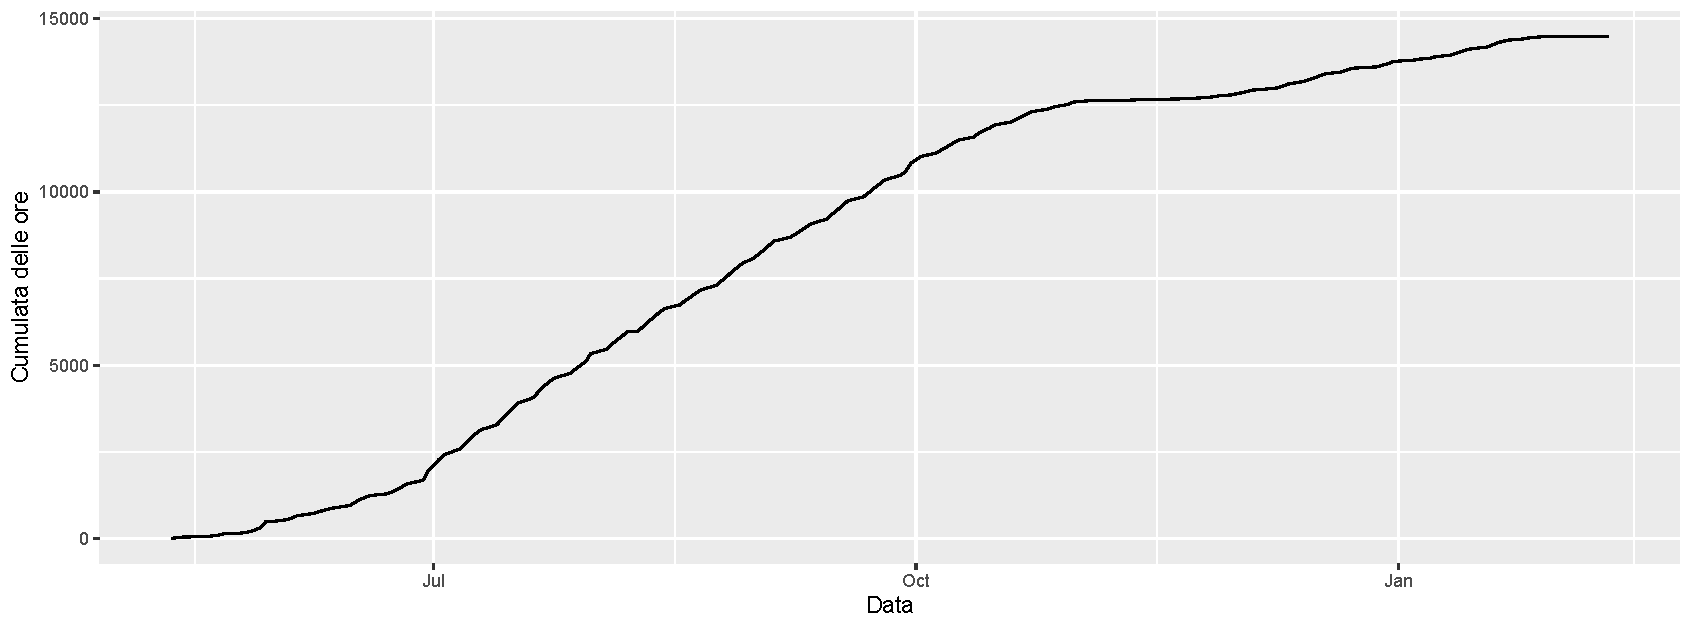
\includegraphics[width = \linewidth]{cumTesla.pdf}
	\caption{Grafico della cumulata delle ore nel tempo}
\end{figure}

\begin{multicols}{2}
	È tuttavia importante sottolineare come i dati non sembrino essere del tutto affidabili, e l'analisi potrebbe quindi essere sfalsata. Analizzando la sovrapposizione temporale delle attività si trovano infatti delle discrepanze.
\end{multicols}

\begin{figure}[H]
	\centering
	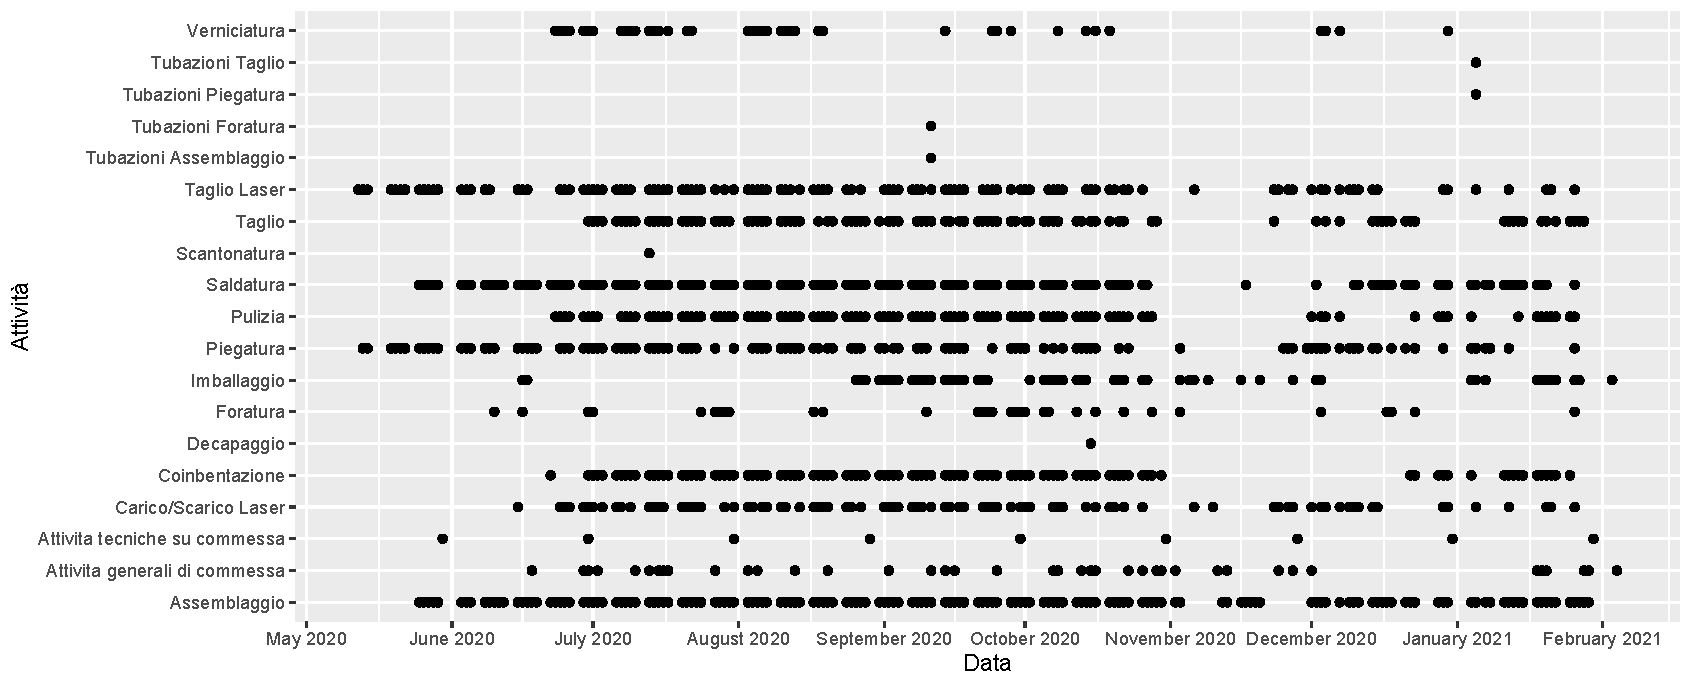
\includegraphics[width = \linewidth]{giorniLavorati.pdf}
	\caption{Giorni in cui si è svolta un'attività. Ogni punto rappresenta che l'attività sull'asse verticale è stata svolta nella data indicata da quello orizzontale.}
\end{figure}

\begin{multicols}{2}
	Per evidenziare questa criticità bisogna porre attenzione ad attività come "Carico/scarico laser" che inizia molto dopo il taglio laser, cosa impossibile essendo la prima un'attività propedeutica alla seconda. Le attività tecniche (ovvero la progettazione) sono invece segnate soltanto nell'ultimo giorno del mese in cui sono state svolte, e la voce include tutte le ore compiute durante quel mese.

	Questo porta l'attenzione su un altro problema importante che colpisce l'azienda, ovvero l'assenza di dati  o la loro scarsa affidabilità. Proprio per questo è stata considerata come opzione l'adozione di moduli ERP che facilitassero la raccolta di dati sui tempi. L'azienda ha infatti contattato due imprese che offrono questi servizi e ha ricevuto dei preventivi che sta ora valutando.
	In particolare le soluzioni proposte consistono nell'installazione di tablet nelle stazioni di lavoro, dotati di un software proprietario che permette di integrarsi con l'ERP che l'azienda utilizza attualmente, fornendo dati precisi sulle ore svolte dai lavoratori e su quale commessa queste sono state impiegate.

	Sebbene questa soluzione potrebbe aiutare l'azienda nel raccogliere dati con una maggiore precisione, è stato ritenuto prioritario concentrarsi sulle logiche gestionali, cambiando le abitudini dei membri dell'impresa verso una gestione migliore delle commesse, acquistando eventualmente in futuro questi software solo se ritenuti utili al fine di semplificare l'utilizzo delle logiche proposte, in particolare in ottica di gestione multi-commessa.

	L’assenza di dati sugli scarti in produzione ha poi portato ad analizzare l’utilizzo di materiali preventivati rispetto a quelli effettivamente acquistati. Alcuni dati emersi risultano strani: in una commessa per esempio sono stati acquistati 40.000 kg di un tipo di lamiera di cui erano richiesti solamente 700 kg e 10.000 kg di una che non era nemmeno stata messa a preventivo. È evidente come un acquisto di 50.000 € di materia prima in più possa avere un impatto significativo sui margini di commessa, evidenziando la necessità d'implementare un sistema migliore di gestione del magazzino e di gestione degli ordini dei materiali.


\section{Creazione del funzionigramma}
	Come è già stato menzionato nella parte introduttiva del documento, le due problematiche principali sono l’assenza di un ruolo di gestione della commessa e di un efficace controllo qualità. Entrambe queste debolezze trovano giustificazione nell’organigramma aziendale, in cui il primo ruolo è completamente assente e il secondo è mal definito, senza assegnare responsabilità e modi di operare alla responsabile della qualità.

	Per migliorare questa situazione si è deciso di creare una nuova versione dell'organigramma, dotata di una chiara attribuzione delle responsabilità per ogni processo, ipotesi di KPI e descrizione della mission di dell'unità organizzativa.

	È stato deciso di mantenere la struttura funzionale già presente in azienda principalmente perché è già vicina alla prassi aziendale e consente una maggiore efficienza di gestione, permettendo ai responsabili di concentrarsi su un solo settore e raggruppando tutto il know-how riguardante quel settore in una sola unità organizzativa. È stato inoltre pensato che la soluzione di gestione della commessa che verrà presentata successivamente potrà aiutare a mitigare gli aspetti negativi della struttura funzionale, come la difficoltà di condivisione degli obiettivi generali, la struttura rigida e verticista e soprattutto i rischi di chiusura tra le funzioni.

	In particolare la nuova struttura organizzativa sarà composta da due funzioni core:

	\begin{itemize}
		\item Operations: Divisa in logistica, produzione e manutenzione
		\item Innovation: Costituita dalle unità organizzative progettazione e commerciale
	\end{itemize}

	È poi stata creata una funzione chiamata amministrazione che racchiude tutte le funzioni di staff dell’azienda, come amministrazione controllo e finanza, human resources, facility management, acquisti e gestione IT.
  La novità principale tra queste è l'introduzione della funzione human resources, che attualmente è in mano al direttore generale dell'impresa che sostanzialmente si occupa soltanto di condurre i colloqui per le nuove assunzioni.
  Creando una funzione a sé stante che si occupi della gestione delle risorse umane, si pone una maggiore enfasi sulla centralità delle persone in azienda, favorendo lo sviluppo e la crescita del personale e la comunicazione interna. 
	Non approfondirò molto la creazione delle altre aree, poiché sono state introdotte solo piccole modifiche rispetto alla prassi già presente in azienda.

	Sono poi state separate due funzioni di supporto completamente nuove per dargli più peso in azienda: gestione qualità e gestione delle commesse. Si noti che al momento in realtà la gestione delle commesse sarà un ruolo e non un'unità organizzativa, e non andrebbe quindi in organigramma. È tuttavia stato deciso di inserirlo comunque perché a tendere esisterà un'unità organizzativa più strutturata che racchiude tutti i project manager.
\end{multicols}

\begin{figure}[H]
	\centering
	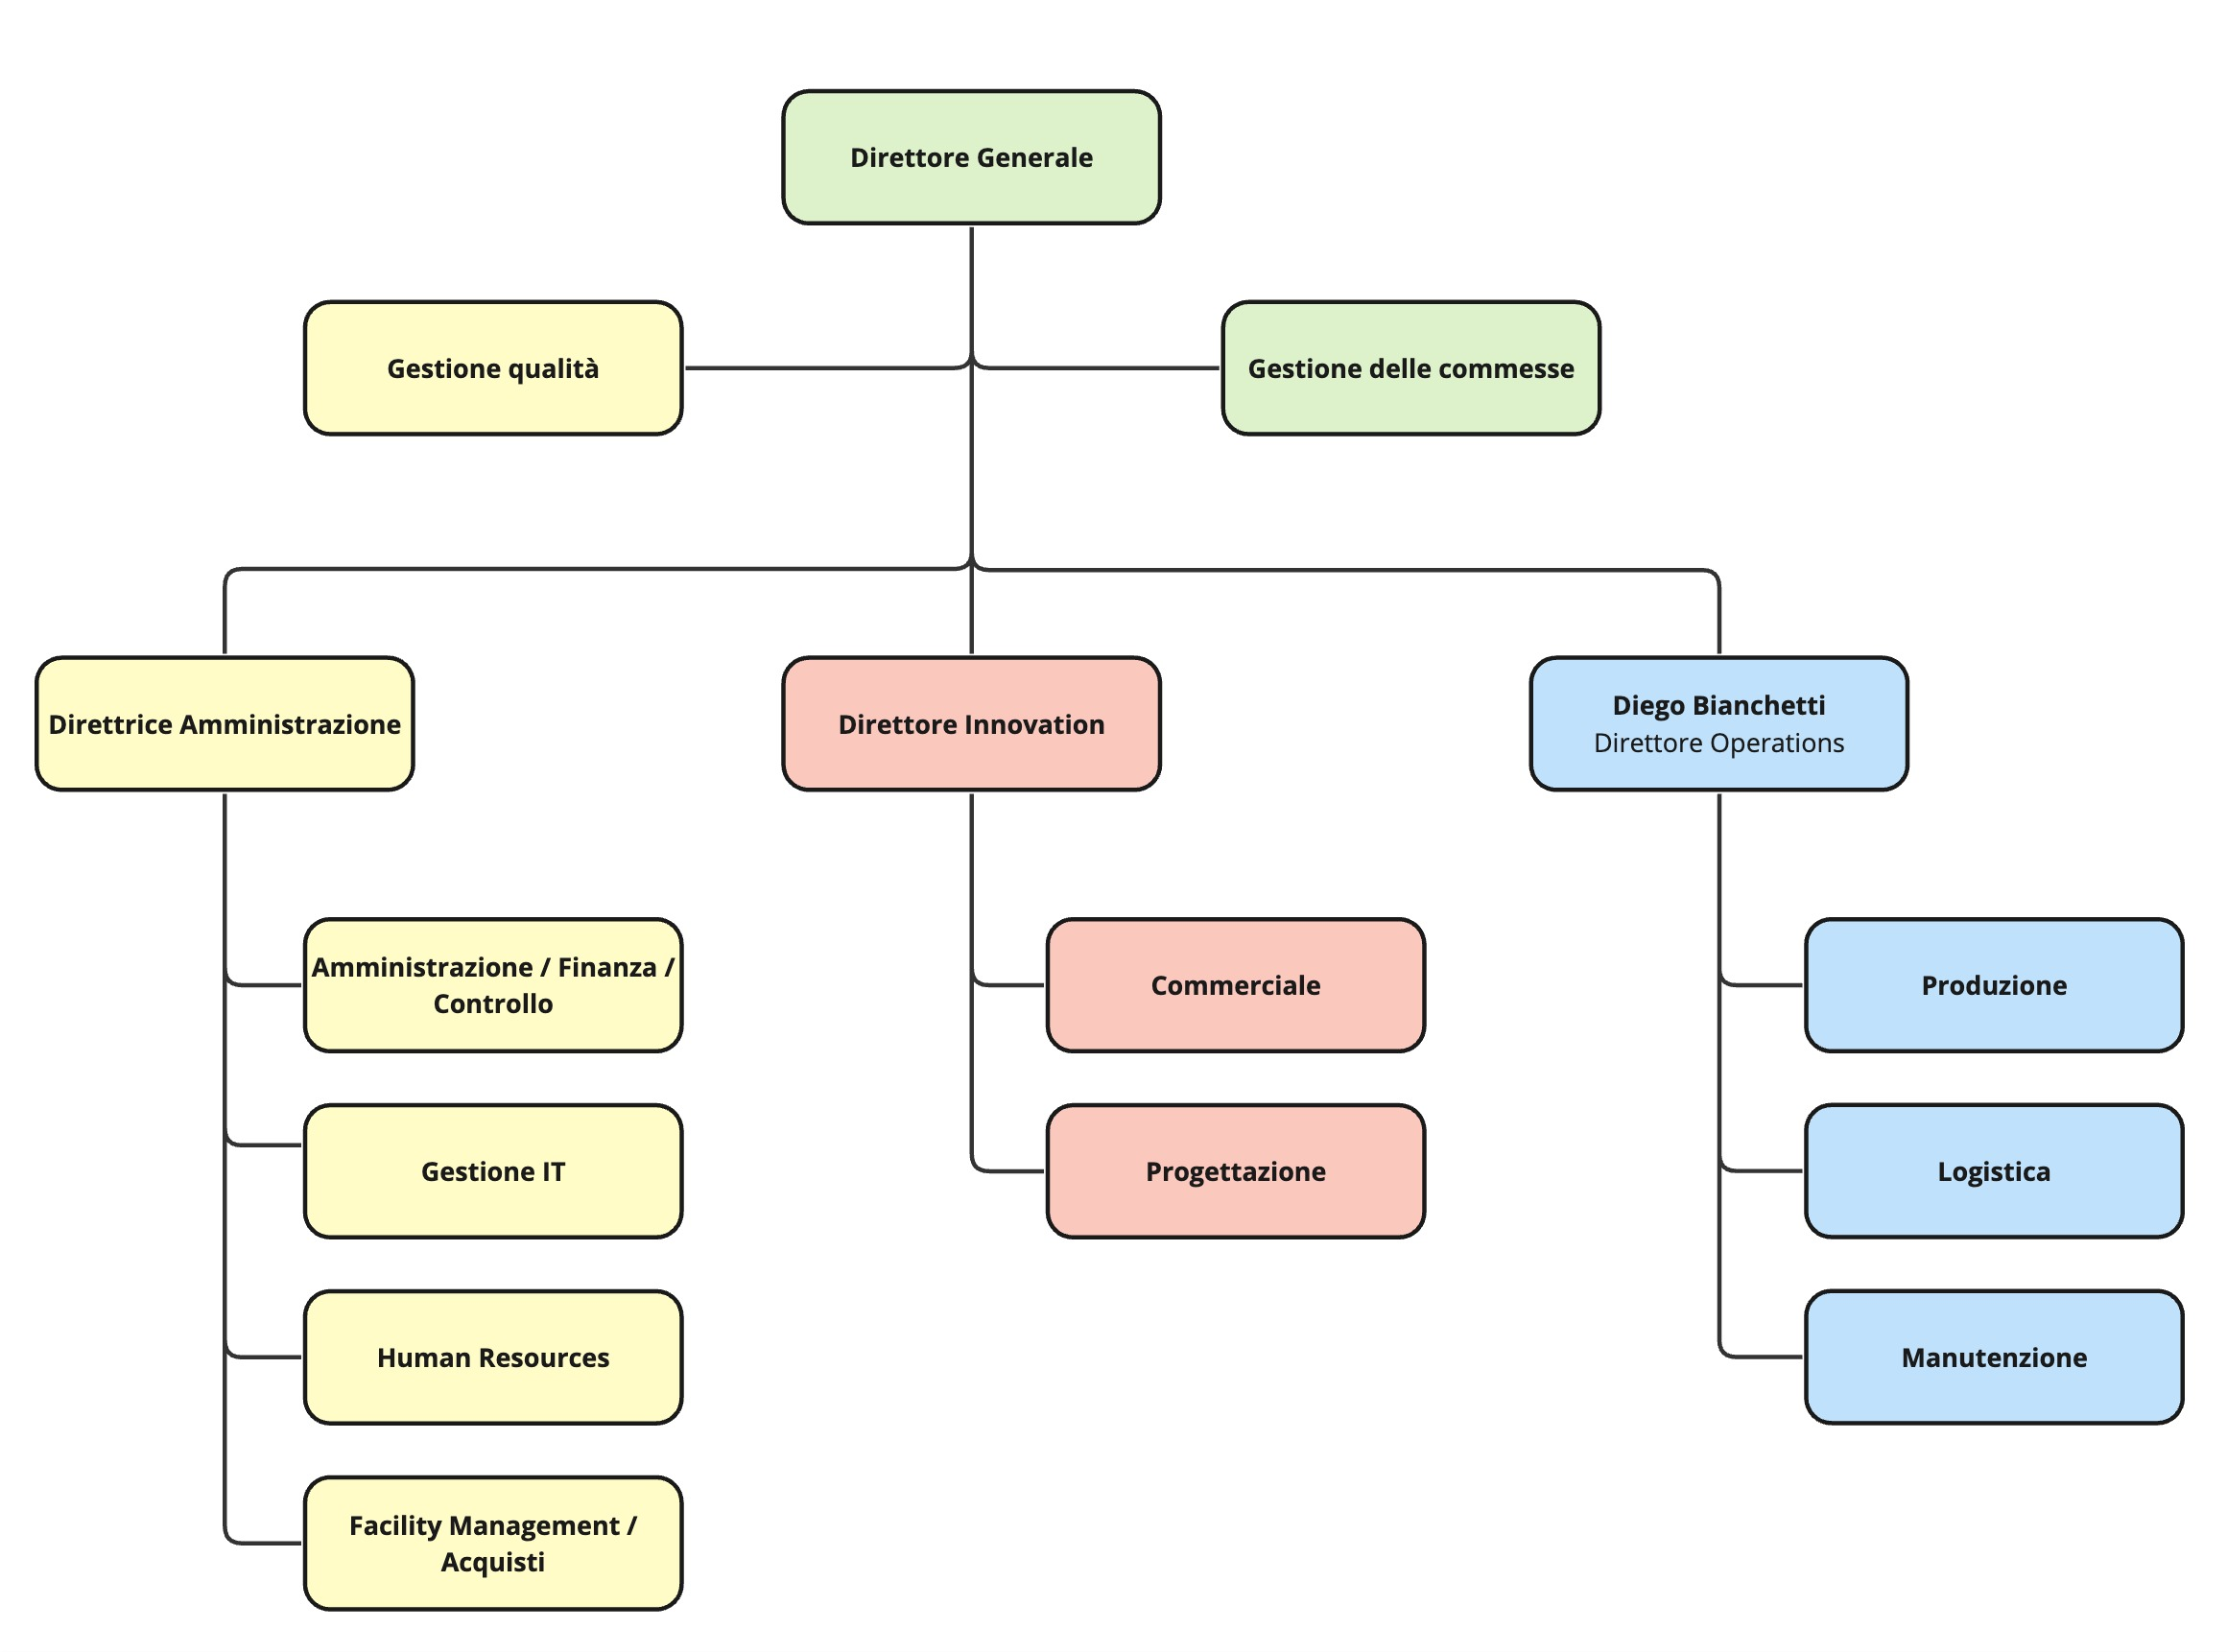
\includegraphics[width = \linewidth]{funzionigramma}
	\caption{Funzionigramma proposto}
\end{figure}

\begin{multicols}{2}
	La funzione gestione qualità ha la responsabilità di presidiare le prestazioni dei processi chiave di Montagna e la soddisfazione dei clienti. Evidenzia le necessità e le opportunità di intervento, indirizzando le azioni di miglioramento, monitorandone i risultati. Per rendere più robusto l’operato di questa funzione è stato deciso che opererà tramite un comitato, composto da membri di tutte le aree aziendali. Così facendo sarà più difficile delegittimare il controllo qualità come è già successo in passato e sarà possibile attribuire meglio le responsabilità per le non conformità avendo competenze specialistiche da ogni funzione.

	Il ruolo del comitato sarà dunque quello di presidiare operativamente la qualità, identificando opportunità di miglioramento, monitorando avanzamenti e risultati e raccogliendo e formalizzando i dati e gli indicatori di qualità. Dovrà inoltre farsi garante della gestione dei controlli richiesti dai clienti e standard di Montagna. I risultati delle precedenti operazioni dovranno poi essere riportati al responsabile della funzione gestione qualità, che si occuperà della formalizzazione e dell’applicazione delle nuove modalità gestionali emerse a valle dei miglioramenti.

  La funzione di gestione della commessa invece, andrà in futuro a racchiudere tutti i project manager presenti in azienda, ovvero coloro che sono responsabili di guidare la realizzazione di ogni commessa acquisita, nel rispetto delle specifiche concordate e di tutti gli obiettivi, quali tempi, margini e qualità. Le responsabilità del project manager sono quelle di:
	\begin{itemize}
		\item Analizzare le specifiche concordate
		\item Definire le risorse necessarie per completare la commessa
		\item Gestire le riunioni di kickoff e controllo avanzamento della commessa
		\item Pianificare le attività evidenziando i rischi e cercando di ridurli
		\item Formalizzare e diffondere le lezioni apprese a fine commessa
		\item Monitorare la soddisfazione del cliente e gestirne le interazioni
	\end{itemize}

	Proposto il funzionigramma e accettato dai soci, è ora responsabilità dei soci operativi definire le risorse apicali e l’impegno atteso, eventualmente assumendo le risorse necessarie e al momento mancanti in azienda, creando così l’organigramma. Sarà allora necessario condurre le opportune attività di formazione per i nuovi ruoli, come gestione della commessa e gestione qualità.

\section{Gestione della commessa}
\subsection{Il visible planning}
	L’approccio che è stato deciso di utilizzare è l’approccio chiamato “visible planning”, nato in Giappone in Nissan e Toyota negli anni '90. Questa metodologia, caratterizzata da strumenti snelli ed efficaci per il project management, punta a coniugare la dimensione tecnica con quella relazionale e organizzativa, migliorando la comunicazione interna e la collaborazione tra i team.

	Sul proprio sito JMAC (Japanese Management Association Consultants) scrive infatti:\\\textit{	“La tradizionale gestione dei progetti di innovazione e sviluppo nuovi prodotti si rivela spesso eccessivamente semplicistica e razionale. Anche l’applicazione di strumenti tradizionali del project management quali il Gantt, il Pert, etc. si conclude spesso in poco più di una sterile esercitazione di pianificazione, che non tiene in considerazione gli aspetti legati alle persone e all’organizzazione”}

	L’obiettivo dell’introduzione di questa metodologia è infatti quello di renderla anche lo strumento principale per migliorare la comunicazione all’interno dell’azienda, andando così a offrire una soluzione indiretta anche alla terza problematica riportata nell’introduzione del presente report. Tramite questo approccio di project management è infatti incoraggiato il lavoro diretto sui meccanismi di comunicazione e relazionali tra i membri del team.

	Il Visible Planning si basa sul principio di “rendere visibili” i contenuti fondamentali del lavoro con particolare attenzione a:

	\begin{itemize}
		\item Obiettivi
        \item Pianificazione delle attività dei team e delle unità coinvolte
		\item Individuazione, analisi e risoluzione di problemi e criticità
	\end{itemize}

	La disponibilità di tutte queste informazioni a tutti coloro che sono parte della commessa attiva una modalità di comunicazione nuova e più naturale, basata sulla collaborazione tra le diverse funzioni aziendali coinvolte e sul rafforzamento del ruolo attivo del management come supporto nella risoluzione dei problemi.
	Anche gli strumenti operativi utilizzati, che verranno descritti più approfonditamente successivamente, puntano a promuovere la collaborazione di tutti coloro che partecipano alle riunioni per un migliore coordinamento e quindi una migliore gestione della commessa.

\subsection{Le fasi}
	\subsubsection{Kickoff}
	Il kick off rappresenta il momento di lancio del progetto gestito tramite il visible planning. Solitamente dura due giorni, ma nel caso di Montagna è stato deciso di ridurne la durata a una sola giornata per via del grande carico di lavoro che l’azienda si trova ad affrontare, eliminando ogni momento non strettamente legato allo sviluppo della commessa. A queste riunioni partecipano, oltre ai project manager, anche persone di tutte le aree aziendali coinvolte sul progetto.

	Il kick off ha i seguenti obiettivi:
	\begin{itemize}
		\item Mettere sul tavolo tutte le difficoltà, le incomprensioni e i rischi che normalmente si generano con un nuovo progetto.
		\item Condividere milestones e macroattività iniziando a compilare i template relativi alla pianificazione di lungo e medio periodo.
	\end{itemize}

	La prima giornata inizia con un’introduzione da parte del management. I partecipanti, suddivisi in gruppi, devono dapprima segnare i problemi che tipicamente vivono durante i progetti, condividendoli poi e raggruppandoli in macrocategorie ed evidenziando i problemi prioritari per ogni categoria. Così facendo si possono comprendere i problemi principali affrontati dagli attori in azienda, evidenziandone relazioni di causa effetto e individuando circoli viziosi da rompere. 

	La seconda fase della giornata di kickoff vede invece come ruolo fondamentale quello del project manager, che spiega a tutti i partecipanti, divisi in base alla funzione di appartenenza, gli obiettivi, le caratteristiche e le tempistiche del progetto. Durante la spiegazione, i coinvolti devono segnare ogni dubbio, domande e perplessità, ai quali il project manager deve poi rispondere laddove possibile. Ogni problema deve poi essere appeso alla “issue board”, un documento con tre colonne (problemi, problemi in risoluzione e problemi risolti). Nella colonna dei problemi sono semplicemente riportate le criticità individuate. Quando questo viene poi spostato nei problemi in risoluzione gli viene allegato il tentativo che si sta provando per risolvere il problema. Nella colonna dei problemi risolti invece è scritto, oltre al problema la soluzione che è stata adottata con il risultato ottenuto. Una volta risolta una criticità è bene che rimanga sulla issue board, in modo che qualora si ripresentasse un problema simile si ha una soluzione efficace già provata, portando a una migliore gestione delle criticità in azienda.

	Conclusa questa prima parte di condivisione, inizia la fase di pianificazione: stilate le milestone di progetto, vengono definite le attività da svolgere nel lungo periodo tramite un template avente sulle righe le funzioni coinvolte e sulle colonne i mesi. Ogni cella conterrà le attività che la funzione deve svolgere in quel mese per raggiungere le milestone in tempo. Qualora ci fossero incongruenze nei piani di due funzioni è bene che vengano risolte ora, eventualmente pianificando attività extra come ricorrere a terzisti per parti di attività che fanno da collo di bottiglia.

	Fatto ciò si passa alla pianificazione di medio termine. Per fare ciò il mese viene suddiviso in settimane, e sulle righe vengono poste le singole risorse da coinvolgere nel progetto. A questo punto bisogna pianificare le attività settimanali di ogni gruppo di lavoro in modo che siano coerenti e permettano di raggiungere gli obiettivi formalizzati durante la pianificazione di lungo termine.

	\subsubsection{Riunioni settimanali}
	Le riunioni sono condotte con frequenza settimanale e sono il principale metodo di controllo avanzamento adottato nel progetto che utilizza la tecnica del visible planning. È fondamentale evidenziare che, al fine di rendere la metodologia il più snella possibile, queste riunioni siano estremamente rapide. Per fare ciò è importante che durante gli incontri di avanzamento si parli soltanto dei problemi che sono stati riscontrati e non di ciò che è stato fatto. Ogni riunione dovrebbe infatti durare un massimo di venti minuti. È opportuno che a queste riunioni partecipino tutti i coinvolti almeno nelle fasi prossime della commessa.

	Una volta al mese invece le riunioni sono un po’ più lunghe, e durante queste si analizzano scostamenti sia in termini di tempi che di budget, discutendo eventuali cambi di pianificazione e soluzioni per ridurre i costi qualora sia necessario. È importante invece che a queste riunioni non partecipi solo chi verrà coinvolto prossimamente nella commessa, ma tutti, in modo che anche chi non prenderà parte al progetto ancora a lungo sia aggiornato sulle criticità e difficoltà affrontate dagli altri.

	\subsubsection{Declaration}
	Dopo circa tre mesi dall’avvio del progetto di introduzione del visible planning è buona norma confrontarsi sugli obiettivi e sullo stato di avanzamento. Questa riunione è composta di brevi presentazioni individuali che descrivono cosa è stato fatto e appreso e cosa verrà fatto in futuro per migliorare. Così facendo si può controllare la percezione in azienda della nuova metodologia, concettualizzando le attività svolte e verificandone l’utilità.

	\subsubsection{Lessons Learnt}
	Una parte fondamentale di qualunque progetto è imparare da ciò che è stato fatto. Esiste quindi una riunione il cui scopo è quello di valorizzare al massimo l’esperienza vissuta, traducendo i problemi riscontrati in spunti per il miglioramento futuro. L’obiettivo di questo tipo di riunione è che dia inizio a un ciclo di miglioramento continuo, che porti a una crescita degli operatori e a una riduzione della paura di comunicare i propri errori che è purtroppo tipica in Montagna.

	È importante che venga evidenziata l’importanza di segnalare più problemi possibili, che porteranno a un miglioramento anche per progetti futuri. Questo incoraggia anche la comunicazione bottom-up, facendo sì che i dipendenti possano comunicare anche i problemi operativi e relazionali che hanno avuto durante il progetto ai direttori, che potranno diventare più coscienti di problematiche che al momento sfuggono, dandogli la possibilità di intervenire direttamente migliorando le condizioni di lavoro per tutti in azienda.

	Gli spunti di riflessione ricevuti durante queste riunioni dovranno poi essere sfruttati al meglio: non basta infatti condurre incontri di lessons learnt, ma è fondamentale che poi ci sia uno studio volto al miglioramento delle criticità, e che le lezioni apprese diventino nuove procedure, modalità operative, suggerimenti di nuovi investimenti come software di supporto e così via.

\subsection{Perché il visible planning}
	Lo scopo principale del lean manufacturing è quello di eliminare quelli che in gergo vengono chiamati "muda", ovvero gli sprechi.
	Taiichi Ohno, ingegnere giapponese considerato padre del Toyota Production System, individuò sette principali muda, che non aggiungono valore al prodotto e devono quindi essere minimizzati:
	\begin{itemize}
		\item Magazzino
		\item Tempi d'attesa
		\item Difetti
		\item Inefficienze di processo
		\item Movimentazioni inutili
		\item Sovrapproduzione
		\item Trasporti
	\end{itemize}

	L'approccio visible planning  può aiutare l'azienda a ridurre questi sprechi facilitando la condivisione delle informazioni e la collaborazione tra le diverse funzioni aziendali, riducendo i tempi d'attesa e migliorando l'efficienza dei processi.
	Attraverso il kickoff iniziale e le riunioni settimanali di avanzamento, tutti i partecipanti sono costantemente aggiornati sugli obiettivi, le attività pianificate e le criticità riscontrate, permettendo di affrontare i problemi tempestivamente e in modo coordinato.
	Grazie a questo migliore coordinamento anche i tempi di attesa dovrebbero essere ridotti.

	La trasparenza offerta dal metodo proposto consente di individuare più rapidamente i difetti e le inefficienze di processo, facilitando la loro risoluzione. La issue board utilizzata durante le riunioni permette di tracciare e risolvere i problemi in modo strutturato, riducendo gli sprechi legati ai difetti e alle rilavorazioni.

	Un altro grande vantaggio di questa metodologia è che andrà a introdurre una logica pull, che attualmente manca.

	Gli altri muda principali non sono invece problematici per Montagna, che lavorando per commessa ha sempre una quantità limitata di materiale a magazzino, costituito principalmente da semilavorati, e non rischia di produrre più del necessario.
	I trasporti sono poi limitati alla consegna del prodotto finito al cliente, senza una gestione di più siti produttivi o magazzini da gestire.

\end{multicols}
